%\documentclass[12pt]{article}
%\documentclass[conference]{IEEEtran}
\documentclass[12pt,fullpage,doublespace]{article}

\usepackage{amsmath,amssymb}    % need for subequations
\usepackage[dvips]{graphicx}   % need for figures
\usepackage{verbatim}   % useful for program listings
\usepackage{color}      % use if color is used in text
%\usepackage{subfigure}  % use for side-by-side figures
\usepackage{hyperref}   % use for hypertext links, including those to external documents and URLs
\usepackage{epsfig}
\usepackage{float}
%\usepackage[top=0.75in, bottom=1in, left=0.625in, right=0.625in]{geometry}
\usepackage{color}
\usepackage{times}
\usepackage{graphicx}
\usepackage{cite}
\usepackage{graphicx,epstopdf}
\usepackage{listings}


\begin{comment}
\pagestyle{empty} % use if page numbers not wanted
\end{comment}
\DeclareMathOperator*{\argmin}{arg\,min}

% above is the preamble

\begin{document}

\begin{center}
UNIVERSITY OF CALIFORNIA\\
\mbox{}\\
LOS ANGELES\\
\mbox{}\\
\mbox{}\\
\mbox{}\\
\mbox{}\\
\mbox{}\\
\mbox{}\\
\mbox{}\\
\mbox{}\\
\mbox{}\\
{\large UV Data Analysis and Navigation}\\
\mbox{}\\
\mbox{}\\
\mbox{}\\
\mbox{}\\
\mbox{}\\
\mbox{}\\
\mbox{}\\
\mbox{}\\
\mbox{}\\
\mbox{}\\
\mbox{}\\
\mbox{}\\
\mbox{}\\
A comprehensive examination report submitted in partial\\
satisfaction of the requirements for the Masters of Science in\\
Computer Science\\
\mbox{}\\
\mbox{}\\
by
\mbox{}\\
\mbox{}\\
Aditya Modi
\mbox{}\\
\mbox{}\\
\mbox{2012}\\
\end{center}
\newpage
\begin{center}
BLANK PAGE
\end{center}
\newpage
The comprehensive examination of Aditya Modi is approved by :\\
\mbox{}\\
\mbox{}\\
\mbox{}\\
\mbox{}\\
\begin{center}
\end{center}
\hfill\line(1,0){150}\\

\hfill Mario Gerla, Committe Chair\\
\mbox{}\\
\mbox{}\\
\mbox{}\\
\mbox{}\\


\hfill\line(1,0){150}\\

\hfill Junghoo Cho\\
\mbox{}\\
\mbox{}\\
\mbox{}\\
\mbox{}\\


\hfill\line(1,0){150}\\

\hfill Miodrag Potkonjak


\null
\vfill
\begin{center}
University of California, Los Angeles\\
\mbox{}\\
2012
\end{center}
\newpage
\begin{center}
DEDICATIONS:\\
To my parents, grandparents and brother\\
for their love and support that got me going through \\
to complete this project.\\
\end{center}
\newpage

\title{\textbf{UV Data Analysis and Navigation}}
\author{\\\bf {Aditya Modi}\\
Department of Computer Science\\
University of California, Los Angeles \\
Los Angeles, CA 90024. \\
adityam@cs.ucla.edu\\
\mbox{}\\
Professor Mario Gerla}


\date{}
\maketitle


\textbf{\normalsize Abstract}- {Pedestrian’s exposure to UV Radiation depends on many factors, most importaant of which are geographic location and environmental properties. UV radiation in moderation is beneficial to human health like production of Vitamin D. However, overexposure to UV Radiation can lead to many health problems including skin cancer. The purpose of this project is to provide user with a path from the source to the destination , that has minimum UV exposure, thus reducing the health risks. UV data is gathered using a circuit which contains sensors for UVA and UVB. Further, statistical analysis is performed on the data. Data analysis is then done to determine what the minimum number of UV samples is to assert the UV exposure on a path. The aim here is to obtain an accuracy of above 75\% for UVA and above 95\% for UVB. A method is also devised to estimate UV data from the neighboring road segments if the number of samples for a given road segment is lesser than the minimum number of UV samples required for analysis. A Web Service is built to cater the developers to use the system in order to get the best path to route a pedestrian with minimum UV exposure. A web application is also built to consume the web service.}\\
\newpage

\section{Introduction}
Scientists have come to a similarly dichotomous recognition that exposure to the ultraviolet radiation (UVR) in sunlight has both beneficial and deleterious effects on human health. UV exposure is beneficial to humans in a optimum amount since it is necessary for the production of Vitamin D in the body. Unlike other essential vitamins, which must be obtained from food, vitamin D can be synthesized in the skin through a photosynthetic reaction triggered by exposure to UV radiation ~\cite{dep1}. So, it is necessary for humans to get an optimum amount of UV exposure. However, over exposure of UV have a lot of bad implications on the body like skin cancer and sun burns. These health effects could have been worsened due to the depletion of the ozone layer resulting in increase in UV radiation \cite{dep2}. The effect on human health of solar UV at the earth’s surface depends on many factors like geographic location and environmental properties.  

The UV spectrum, shown in Figure \ref{fig:uvSpectrum} is divided into three wavelengths: UVA 315-400nm, UVB 280-315nm and UVC 200-280nm \cite{dep4}. The ozone layer of earth blocks UVC radiations where as UVA and UVB radiations pass through the atmosphere. UVA radiation penetrates deeply into the skin, where it can contribute to skin cancer indirectly via generation of DNA-damaging molecules such as hydroxyl and oxygen radicals. Sunburn is caused by too much UVB radiation; this form also leads to direct DNA damage and promotes various skin cancers. Erythema is caused primarily by the UVB \cite{dep3}. It causes reddening of the skin by damaging the epidermal layer. The amount of UV radiation that is absorbed or scattered is determined by a number of factors. For measurement of UV Radiation, there is a metric called UV index \cite{dep5}. 
\begin{figure}
\begin{center}
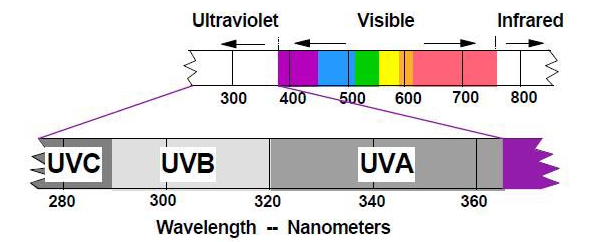
\includegraphics[scale=0.40]{uvSpectrum.png}
\caption{\small \sl UV Spectrum\label{fig:uvSpectrum}}
\end{center}
\end{figure}


Since over exposure of UV on humans has several adverse effect, exposure to UV radiation should be avoided. The paper highlights a web service to route users through routes with minumum UV exposure and thus reducing the amount of UV exposure on pedestrians. It also showcases a prototype to consume the web service by building a web application. 

In order to estimate the UV levels on a route, analysis was done in order to determine minimum number of samples necessary to assert the UV levels on a particular route. The analysis plays a crucial role in the navigation application since there needs to be a certain confidence in estimating the UV levels on a particular route. Another interesting problem that is discussed in the paper is to estimate the UV on a route when the number of samples are less than the actual number of samples required. The UV level in these cases is estimated from the UV levels of the neighbors. Using the results mentioned in ~\cite{uvguardian}, it is resonable to estimate the UVA accuracy to 75\% and UVB accuracy to 95\%. 

\newpage
\section{Approach}
Work is mainly divided into the following parts:
\begin{itemize}
\item{Route Selection}
\item{Sensor Device Selection}
\item{Data Collection}
\item{Data Analysis}
\item{Web Service Development}
\item{Navigation Web Application}
\end{itemize}
For the project to be a success, the most crucial part is selection of the route for the experiment. The route that is selected needs to have a good mix of trees, buildings and open spaces. A major criteria was to also select a path which has alternate routes so that decision on suggesting a route can be taken by comparing the options based on the UV levels. After the route selection, a selection was to be made for selecting the devices to collect the UV data. A requirement for sensor selection was that device should have sensors to measure both UVA and UVB data. Also there needs to be an interface to transfer the data collected to the computer.  A GPS device is also necessary to keep a track of the latitude and longitude points where the UV data is collected.  

After the data was collected, analysis was done on the data to determine the minimum number of samples necessary to assert the level of UV on a particular route. After the analysis is completed, a web service is developed to incorporate the analysis done so far, and help the developers to create platform independent navigation system on top of the system created. The main idea being the users of the application uploading data to the common server and the web service provides an API to the external world developers. Finally, a web application was also created to consume the web service and provide as a basis for other application developers. 
\newpage
\section{Implementation}
\subsection{Route Selection}
Selecting a route was extremely crucial for the project since UV exposure is affected by geographic and environment properties like trees and buildings. A route should be selected with a good balance of open spance, trees, buildings, and a mixture of all previously mentioned objects. After guaging different route options, a route was selected around UCLA area which had a mix of open space, buildings and trees.  Our source was 606 Levering Ave and destination was 11020 Kinross Ave ~\ref{fig:Route}.  The alternate routes were as follows
 \begin{itemize}
\item  Via Veteran Ave 
\item Via Levering Ave and Gayley Ave
\item Via Weyburn Ave
 \end{itemize}
Veteran Ave route had a good mix of buildings and trees, while Levering Ave/Gayley Ave and Weyburn Ave routes had a good mix of buildings and open spaces. 
\begin{figure} [hb] 
\begin{center}  
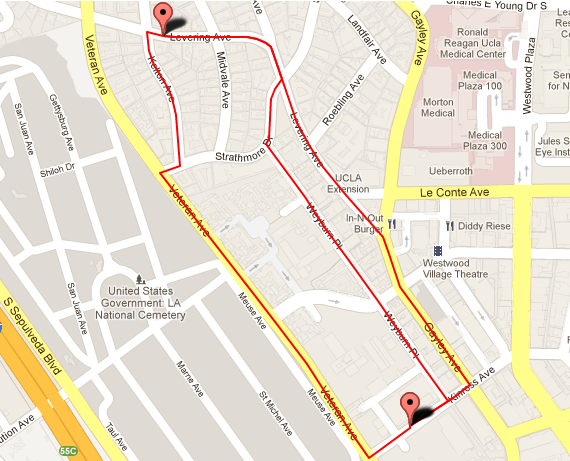
\includegraphics[scale=0.4]{allRoutes.png}
\caption{\small \sl Routes taken for doing the analysis.\label{fig:Route}}  
\end{center}  
\end{figure} 
\subsection{Sensor Device Selection}
Data collection had two main components, UV readings and GPS readings. For UV Readings, a sensor built at UCLA was used ~\ref{fig:uvSensor}. The reason for selecting this sensor was the fact that all our requirements were satisfied. The device had 2 sensors for measuring UVA  UVB each. The units of data output is $mW/nm^2$. The device also had a bluetooth which facilitated transfer of data from the device to a computer. Since there was no GPS device built on the UV sensor, Android device was used to collect GPS readings. After guaging various options for a GPS software on the android market, GPS logger software ~\ref{fig:gpsLogger} was finally selected to log the GPS data since it was very flexible and provided different options to log the data. GPS logger used to log the GPS readings, which were at a later stage merged with the UV sensor readings to get the UV exposure at specific latitude and longitude points. 
\begin{figure}
\begin{center}
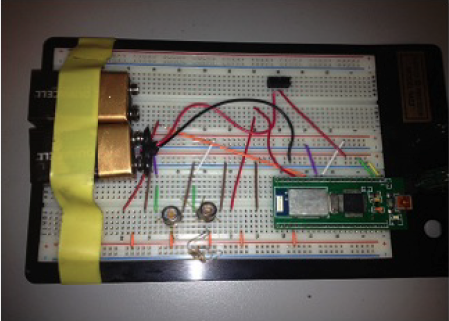
\includegraphics[scale=0.55]{uvSensor.png}
\caption{\small \sl Sensor to collect UV Data.\label{fig:uvSensor}}
\end{center}
\end{figure}
\begin{figure}
\begin{center}
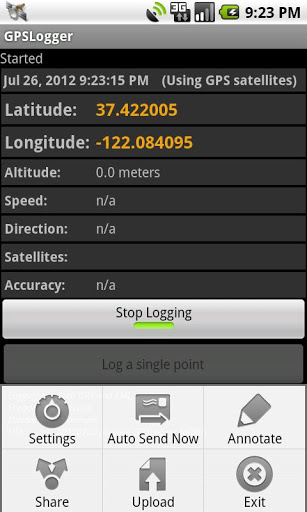
\includegraphics[scale=0.40]{gpsLogger.png}
\caption{\small \sl Software to collect GPS Data.\label{fig:gpsLogger}}
\end{center}
\end{figure}

\subsection{Data Collection}
For collecting the readings, actual walks were done on the selected route ~\ref{fig:Route}. The walks were done by holding the sensor device, a laptop to transfer the readings and an android phone to collect the GPS readings. Readings were taken between 9a.m. and 11a.m. on couple of sunny days with clear sky. Protection from the sun rays may be different on different sides of the road depening on height of the buildings, presense of trees, time of days etc. Thus, readings were taken by walking on both sides of the road wherever possible. Figure ~\ref{fig:dataPoints} shows a plot of points where readings were taken by walking along the road.
\begin{figure}
\begin{center}
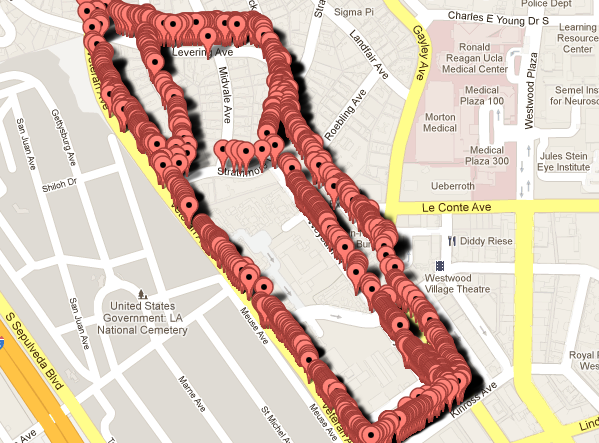
\includegraphics[scale=0.35]{dataPoints.png}
\caption{\small \sl Data points with UV Readings.\label{fig:dataPoints}}
\end{center}
\end{figure}

\subsection{Data Analysis}
\subsubsection{Data Cleansing}
Data cleansing is the most important step of any project where data analysis is involved since analysis can only be performed on clean data and that noisy data should be removed. There were UV readings taken by one device and the GPS readings were taken by another device.So, a script was written to merge the readings so that exact UV readings were collected on the logged GPS points. The UV sensor device sends raw readings which are unreadable by humans. A sample of the raw readings is shown in Fig: \ref{fig:rawReadings}.\begin{figure}
\begin{center}
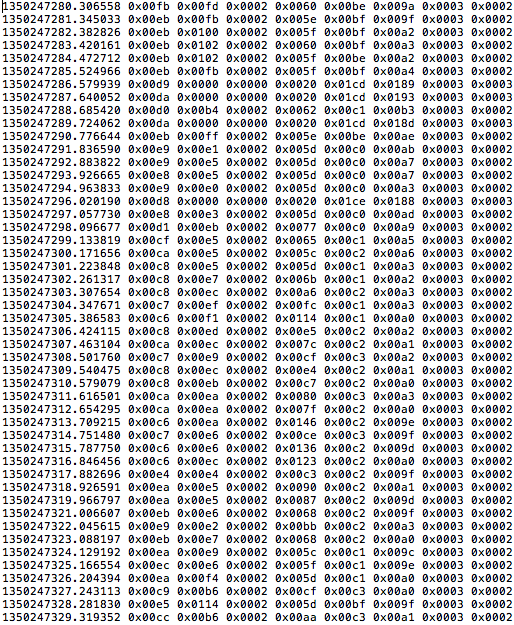
\includegraphics[scale=0.45]{rawReadings.png}
\caption{\small \sl Raw Sensor Readings\label{fig:rawReadings}}
\end{center}
\end{figure} A script  is written to transform these raw readings to humanly readable readings. The readings then contains the UV data at each second. There are four files produced by running the script. A sample of the data is shown in Fig \ref{fig:transformedData}.\begin{figure}
\begin{center}
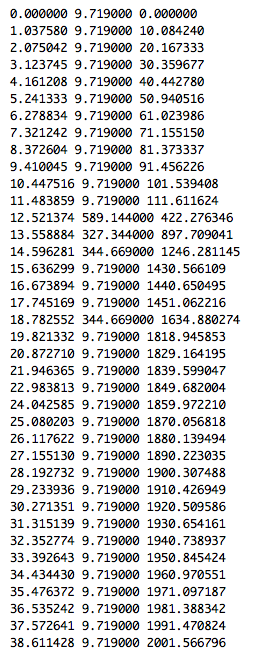
\includegraphics[scale=0.45]{transformedData.png}
\caption{\small \sl Transformed Sensor Readings\label{fig:transformedData}}
\end{center}
\end{figure}. The first column indicates seconds, the second indicates UV readings and the third column hold cumulative UV readings. The GPS readings from the GPS logger software are shown in Fig \ref{fig:gpsReadings}. 
\begin{figure}
\begin{center}
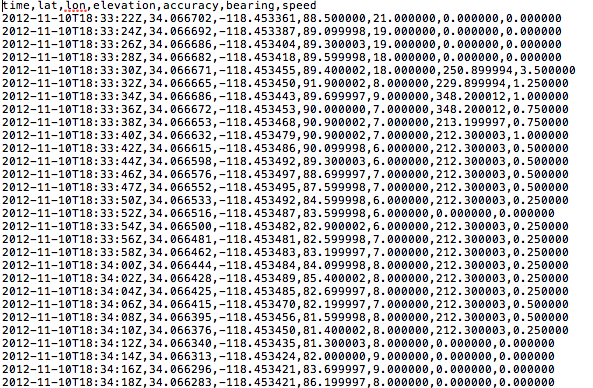
\includegraphics[scale=0.45]{gpsReadings.png}
\caption{\small \sl Raw GPS Readings\label{fig:gpsReadings}}
\end{center}
\end{figure} which hold data for time, latitude, longitude, alevation, accuracy, bearing and speed. 
A scipt is written to join the GPS sensor readings and UV sensor readings. A sample of readings after joining the GPS readings and UV Sensor readings is shown in Fig \ref{fig:joinedReadings}.\begin{figure}
\begin{center}
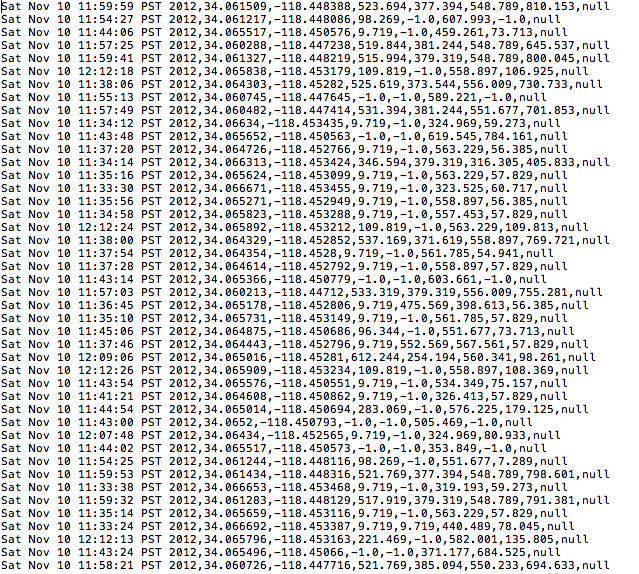
\includegraphics[scale=0.45]{joinedReadings.png}
\caption{\small \sl UV and GPS readings joined\label{fig:joinedReadings}}
\end{center}
\end{figure}. The first column hold data for time, latitude, langitude, UVA1, UVA2, UVB1, UVB2. Also, there were couple of sensors for both UVA and UVB each. So the data was analyzed to determine which of the two sensors readings were more reliable. After careful analysis, one of the two sensors was taken into consideration. As seen in the Fig \ref{fig:dataAnalysis}, a correlation is obervered between first sensors of UVA and UVB. Hence, reeadings from first sensors for both UVA and UVB are considered and readings from other sensors are discarded. There were also some random erroneous readings reported for the sensors sometimes which were discarded. After perfoming all of the above mentioned steps, the data was clean and ready for analysis.
\begin{figure}
\begin{center}
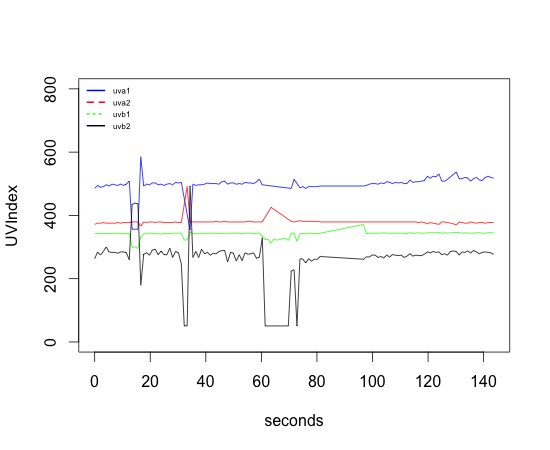
\includegraphics[scale=0.45]{dataAnalysis.png}
\caption{\small \sl UV Sensor Data Readings\label{fig:dataAnalysis}}
\end{center}
\end{figure}



\subsubsection{Determining minimum number of sample points}
The main aim of the project is to suggest the best route to the user out of the many routes options he could take. After carefully considering many options online, Open Street Maps \cite{openStreetMap} and Goolge Maps \cite{googleMapsOriginal} were the good options to be considered. The choice of selecting Google Maps was the fact that no efforts would have to me made for calculating the actual navigation route since there are many robust API's available which good be directly used out of the box. The only programming effort was required to parse the data and selecting only the information which was relevant for the project. 

\begin{figure}
\begin{center}
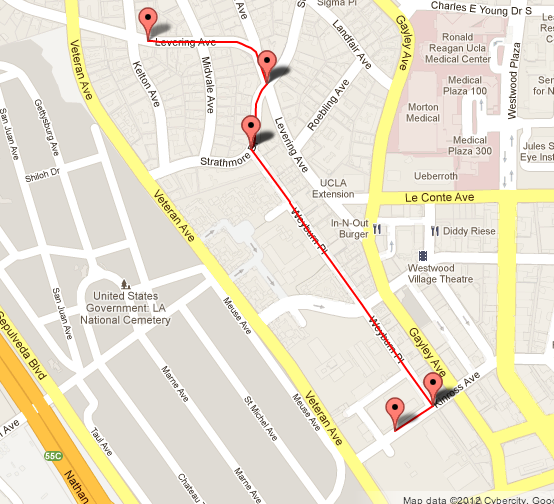
\includegraphics[scale=0.35]{stepsInALeg.png}
\caption{\small \sl Steps in a single Leg.\label{fig:stepsInALeg}}
\end{center}
\end{figure}
\begin{figure}
\begin{center}
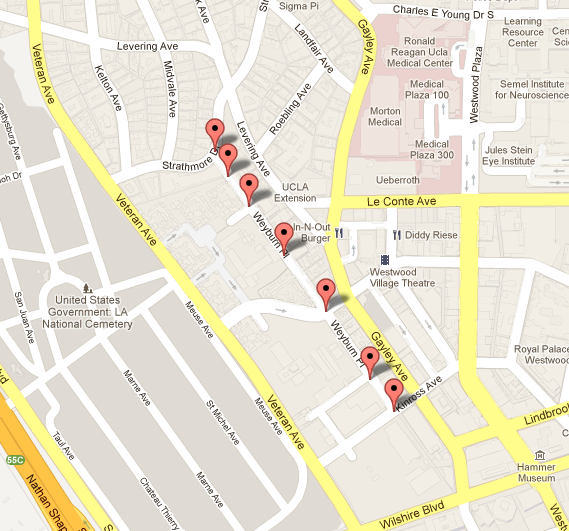
\includegraphics[scale=0.35]{segmentsInAStep.png}
\caption{\small \sl Segments in a single Step.\label{fig:segmentsInAStep}}
\end{center}
\end{figure}

In order to determine the various alternate route options that can be taken to travel from source to destination, Google Maps \cite{googleMapsOriginal} data is used. Open Street Maps option was also considered. Google Maps returned alternate route options when source and destination locations were passed where as in Open Street Maps, the output was in form of the nodes en route to the destination. There is a database of nodes on any path which is returned by Open Street Maps. Since alternate paths were necessary in this project, google maps was used. Google Maps returns the various routes that can be taken which are called as {\it Legs} and the various sections of the roads that changes are called as {\it Steps}. In the route selected for the experiment, each of the red lines in Figure ~\ref{fig:Routes} indicate each leg and each of the red lines between the markers in Figure ~\ref{fig:stepsInALeg} indicate each step. Minimum number of points needed to assert the UV level with a certain confidence was to be found. Analysis was initially done by taking one step and finding the number of points required on that step. However after realizing that the step was too big to perform analysis, decision was made to break each step into smaller segments. After analyzing various options an Open Street Map API  \cite{openStreetMapsDirections} was used. When passed two end points, the API returns all the nodes in its database which come in between the end points. Thus, a pair of nodes would form a segment. Again, scripts were written to parse the data and extracting the information required for the project. Figure ~\ref{fig:segmentsInAStep} indicates segments within a single step. 



Data is analyzed to determine the minimum number of points required to get the accuracy of UVA above 75\% and accuracy of UVB above 95\%. The accuracy limits are selected from \cite{uvguardian} since extensive research was done and also the sensor used was the same one as used in this experiment. Bootstrapping method is used to determine the minimum number of points. Bootstraping works as follows:
\\
\begin{center}
{ 	\boxed{
		\begin{array}{l}
			\text{1. Take the average of all the points on a particular }
		\\ \quad	\text{  segment which would become our actual average }
		\\    \text{2. Select one point randomly}
		\\    \text{3. Calculate the accuracy with respect to the actual}
		\\ \quad	\text{averge}
		\\	\text{4. Select one more point randomly}
		\\	\text{5. Take the avegare of all the points selected till now}
		\\    \text{6. Calculate the accuracy with respect to the actual}
		\\ \quad	\text{ averge}
		\\	\text{7. Repeat from Step 4 till desired accuract is achieved}

		\end{array}
}

\begin{center} 
{\small \sl Algorithm for Boostraping \\}
\end{center} 
}
\end{center}
\newpage
\lstset{caption=R Code for Bootstraping,breaklines=true, tabsize=4, frame=single}
\begin{lstlisting}
route <- read.csv("route.txt", header=TRUE  , sep=",")
for(noOfSample in 1:10){  
  trueMean = mean(route$uvb)
  uvb = route$uvb #getUVB Readings
  uvbReadingsVector <- vector()
  for(i in 1:10){
    uvbSample = sample(uvb,noOfSamples)
    sampleMean = mean(uvbSample)
    accuracy =  abs((trueMean-sampleMean)/ sampleMean*100)
  }
}\end{lstlisting}

Bootstrapping method is chosen since the distribution is completely random and the readings along the segments are not consistent. Bootstrapping is the best method in these cases. For analysis variety of segments are covered by considering different road segments at different orientations and different length of segments. 

\newpage
Detailed analysis of one of a few segments was performed. The segments are considered as follows.
\begin{center}
Segment 1 as seen in Fig. ~\ref{fig:veteranSatellite}. \\
Start Point:  34.060067, -118.449498\\
End Point:  34.058945, -118.44864. \\
Total length of the segment was 480 ft.\\
Time of Day: Between 9am and 10am\\
\begin{figure}[h]
\begin{center}
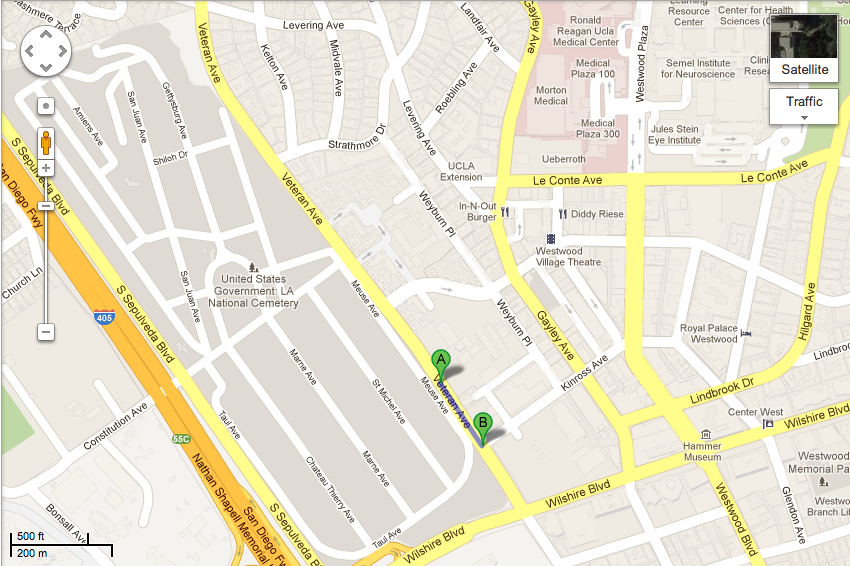
\includegraphics[scale=0.32]{veteranMap.png}
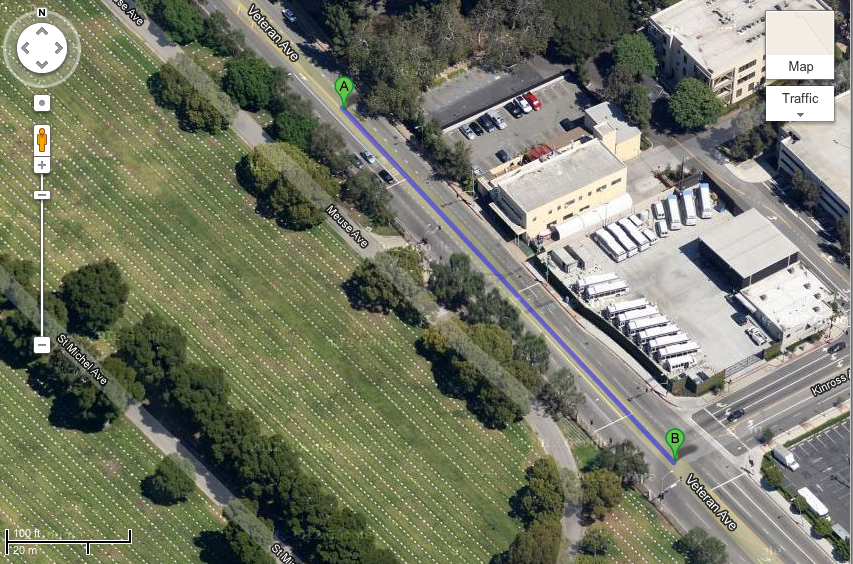
\includegraphics[scale=0.32]{veteranSatellite.png}
\caption{\small \sl Sample selected segment map view}\label{fig:veteranSatellite}
\end{center}
\end{figure}
\end{center}
\newpage
\begin{table}
\centering
\begin{tabular}{|c|c|c|}
\hline
No of Readings & UVA Accuracy & UVB Accuracy \\
\hline 
1 & 72.03039 & 93.37286\\
\hline
2 & 72.84915 & 93.7059 \\
\hline
3 & 73.27921	& 94.36731\\
\hline
4 & 78.09173	& 94.94913\\
\hline
5 & 76.75012 & 95.06996 \\
\hline
6 & 77.60953 & 97.47088 \\
\hline
7 & 78.30137 & 97.91901\\
\hline
\end{tabular}
\caption{\small \sl Accuracy table for bootstraping}\label{seg1accuracy}
\end{table}


\begin{figure}
\begin{center}
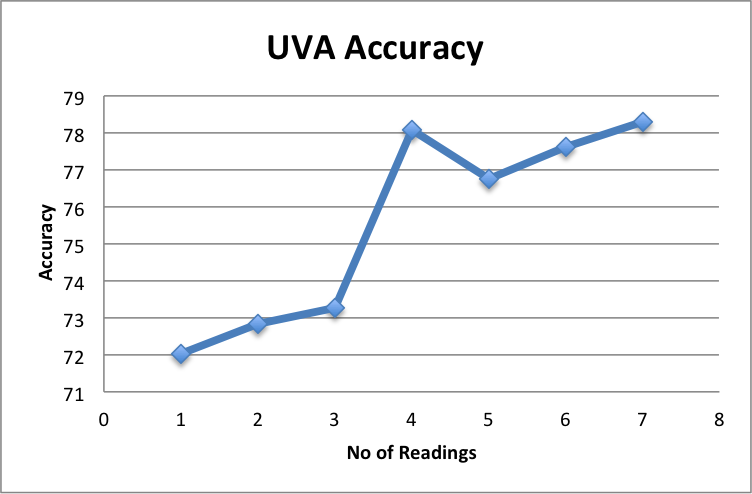
\includegraphics[scale=0.5]{uvaAccuracy.png}
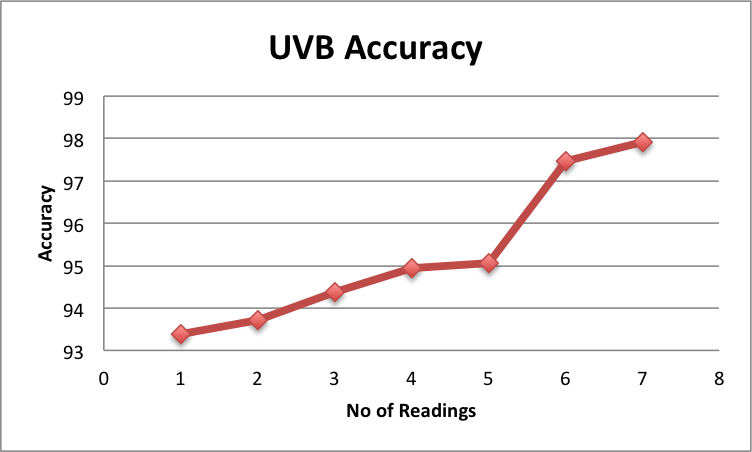
\includegraphics[scale=0.55]{uvbAccuracy.png}
\caption{\small \sl Accuracy v/s No of Readings for UVB}
\label{fig:lessReadings}
\end{center}
\end{figure}


As observed from the table \ref{seg1accuracy} that UVA takes 4 samples to reach the accuracy of 75\% and UVB take 4 readings to reach the accuracy of 95\%. 
\newpage


\newpage
\begin{center}
Segment 2 as seen in Fig. ~\ref{fig:segment2}. \\
Start Point:  34.065270,-118.454607\\
End Point:  34.065948,-118.454169\\
Total length of the segment was 180 ft.\\
Time of Day: Between 9am and 10am\\
\begin{figure}[h]
\begin{center}
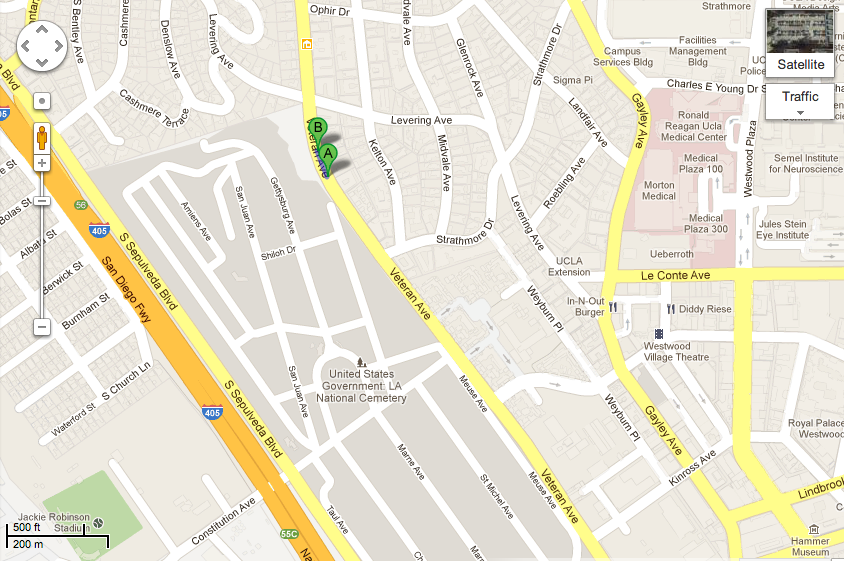
\includegraphics[scale=0.32]{segment2a.png}
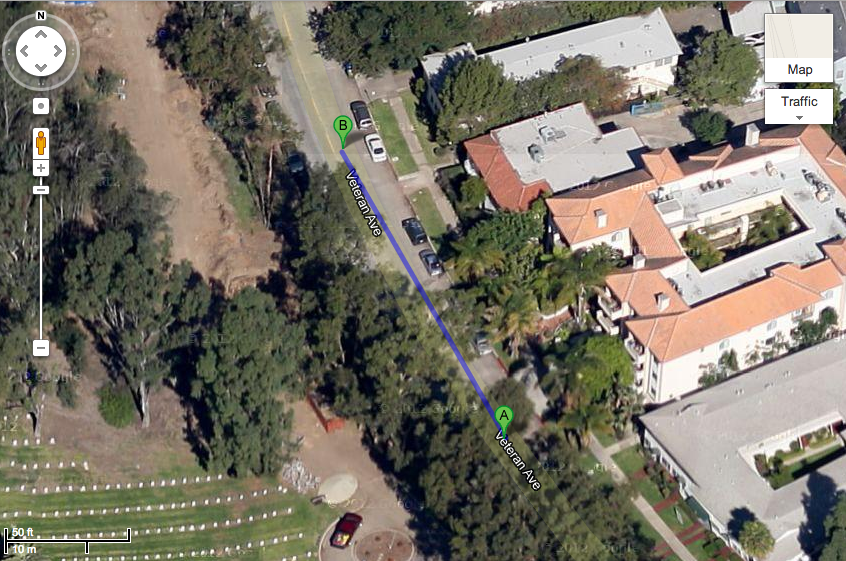
\includegraphics[scale=0.32]{segment2b.png}
\caption{\small \sl Sample selected segment map view}\label{fig:segment2}
\end{center}
\end{figure}
\end{center}
\newpage
\begin{table}
\centering
\begin{tabular}{|c|c|c|}
\hline
No of Readings & UVA Accuracy & UVB Accuracy \\
\hline 
1 & 62.33563 & 90.8751\\
\hline
2 & 68.69139 & 95.34372\\
\hline
3 & 71.9053 & 96.88052\\
\hline
4 & 83.7723 & 96.1235\\
\hline
5 & 75.60744 & 95.95051\\
\hline
6 & 78.77724 & 97.39062\\
\hline
7 & 78.30137 & 97.96218\\
\hline
\end{tabular}
\caption{\small \sl Accuracy table for bootstraping}\label{seg2accuracy}
\end{table}


\begin{figure}
\begin{center}
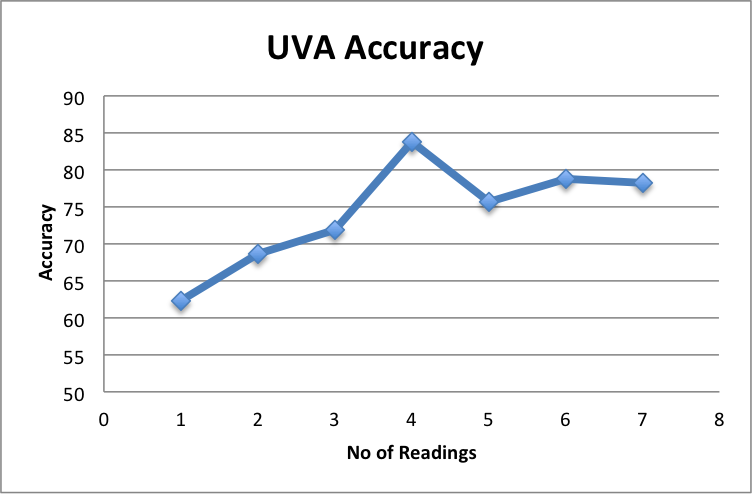
\includegraphics[scale=0.5]{segment2uva.png}
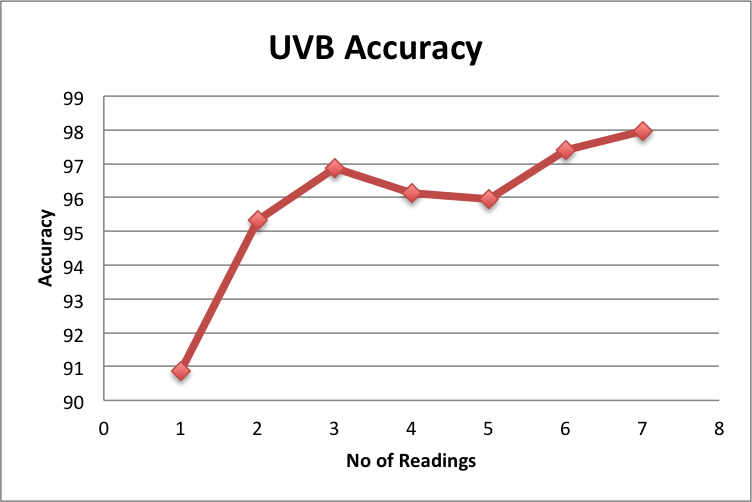
\includegraphics[scale=0.5]{segment2uvb.png}
\caption{\small \sl Accuracy v/s No of Readings for UVB}
\label{fig:lessReadings}
\end{center}
\end{figure}


As observed from the table \ref{seg2accuracy} that UVA takes 4 samples to reach the accuracy of 75\% and UVB take 2 readings to reach the accuracy of 95\%. 
\newpage\newpage
\begin{center}
Segment 3 as seen in Fig. ~\ref{fig:segment3}. \\
Start Point: 34.064022,-118.449589\\
End Point:  34.064489,-118.449965 \\
Total length of the segment was 200 ft.\\
Time of Day: Between 9am and 10am\\
\begin{figure}[h]
\begin{center}
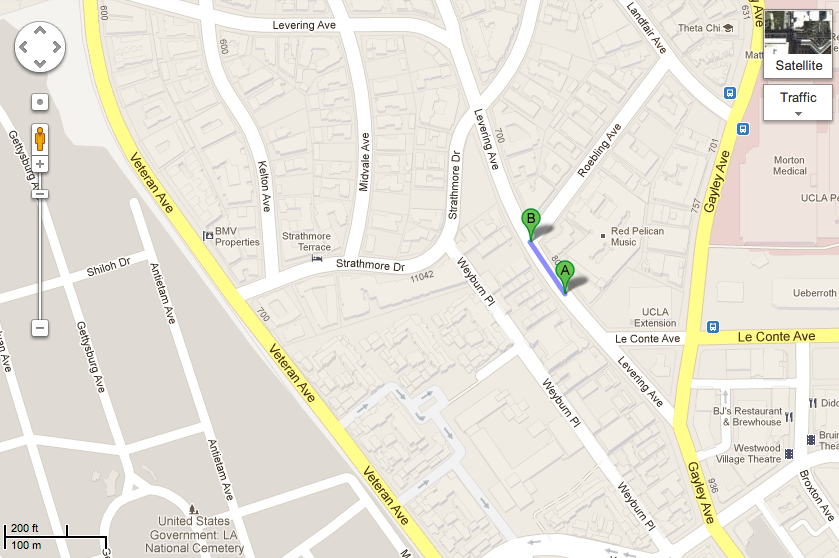
\includegraphics[scale=0.32]{segment3a.png}
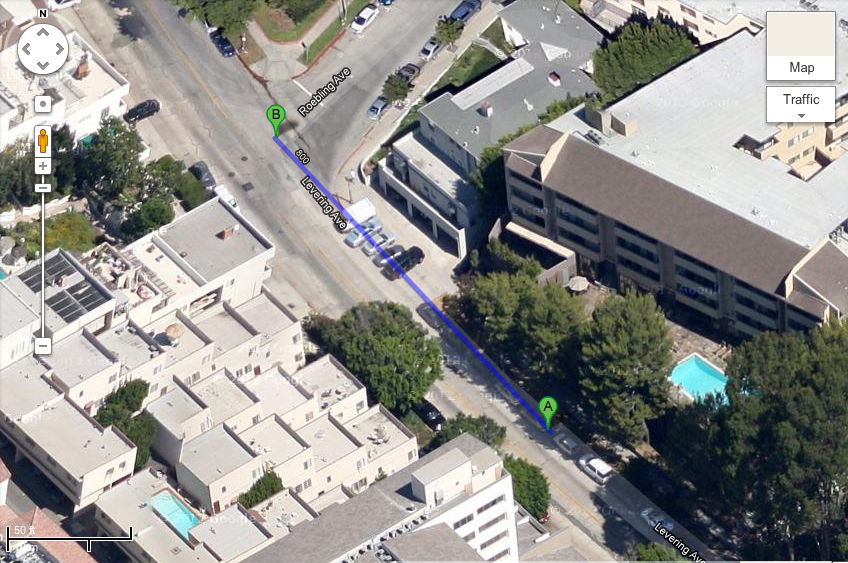
\includegraphics[scale=0.32]{segment3b.png}
\caption{\small \sl Sample selected segment map view}\label{fig:segment3}
\end{center}
\end{figure}
\end{center}
\newpage
\begin{table}
\centering
\begin{tabular}{|c|c|c|}
\hline
No of Readings & UVA Accuracy & UVB Accuracy \\
\hline
No of Readings & UVA Accuracy & UVB Accuracy \\
\hline 
1 & 65.33298 & 90.0156\\
\hline
2 & 62.29749 & 88.62024\\
\hline
3 & 66.94044 & 95.30881\\
\hline
4 & 87.81089 & 95.66149\\
\hline
5 & 77.13757 & 97.265371\\
\hline
6 & 87.79633 & 96.34902\\
\hline
7 & 93.55506 & 97.49347\\
\hline
\end{tabular}
\caption{\small \sl Accuracy table \ref{seg3accuracy} for bootstraping}\label{seg3accuracy}
\end{table}


\begin{figure}
\begin{center}
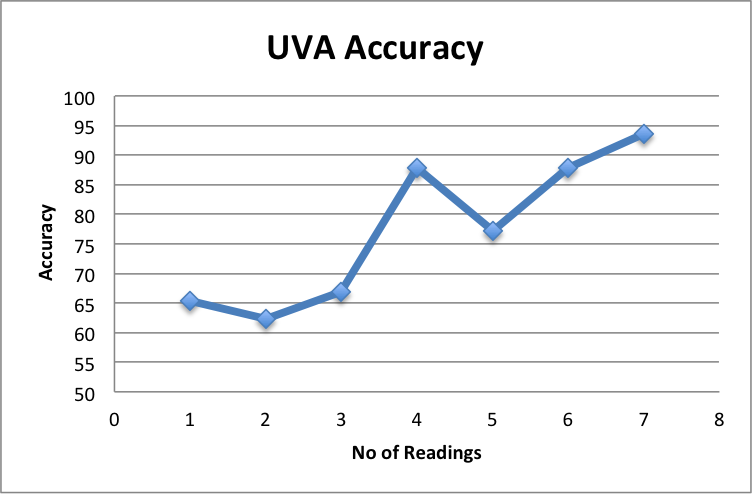
\includegraphics[scale=0.5]{segment3uva.png}
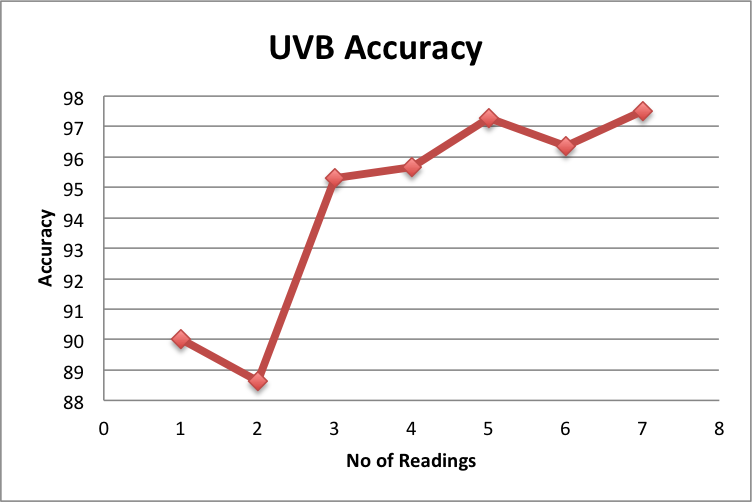
\includegraphics[scale=0.5]{segment3uvb.png}
\caption{\small \sl Accuracy v/s No of Readings for UVB}
\label{fig:lessReadings}
\end{center}
\end{figure}


As observed from the table that UVA takes 6 samples to reach the accuracy of 75\% and UVB take 3 readings to reach the accuracy of 95\%. 
\newpage\newpage
\begin{center}
Segment 4 as seen in Fig. ~\ref{fig:segment4}. \\
Start Point:  34.059344,-118.448027\\
End Point:  34.058979,-118.448648\\
Total length of the segment was 233 ft.\\
Time of Day: Between 9am and 10am\\
\begin{figure}[h]
\begin{center}
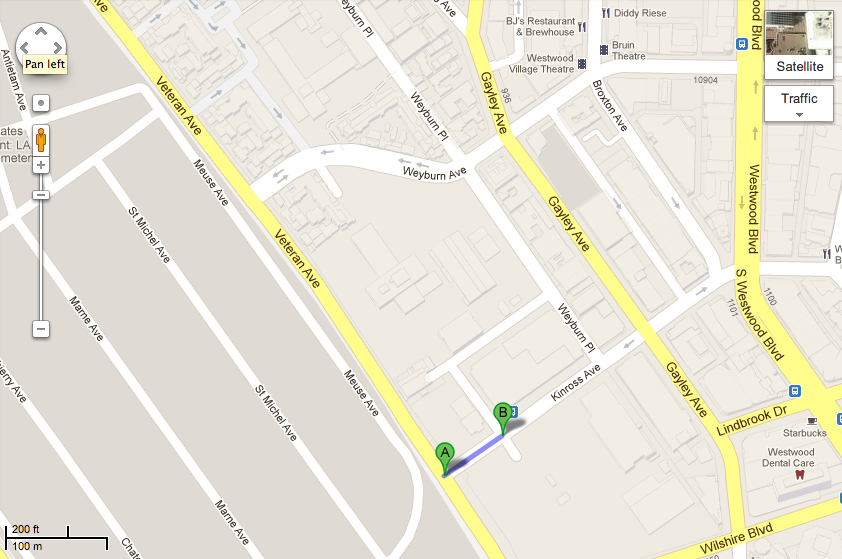
\includegraphics[scale=0.32]{segment4a.png}
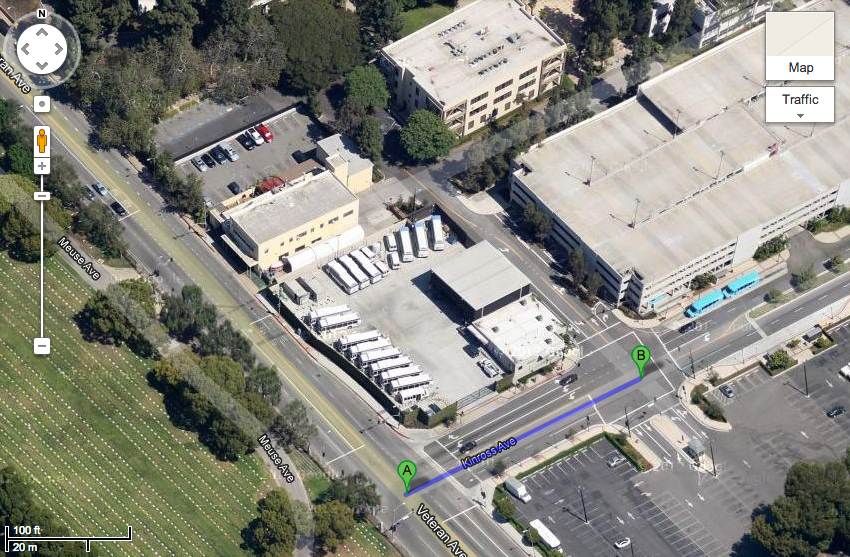
\includegraphics[scale=0.32]{segment4b.png}
\caption{\small \sl Sample selected segment map view}\label{fig:segment4}
\end{center}
\end{figure}
\end{center}
\newpage
\begin{table}
\centering
\begin{tabular}{|c|c|c|}
\hline
No of Readings & UVA Accuracy & UVB Accuracy \\
\hline 
1 & 65.7383 & 91.02471\\
\hline
2 & 71.87201 & 91.05025\\
\hline
3 & 75.28261 & 93.0015\\
\hline
4 & 75.29943 & 94.89313\\
\hline
5 & 82.68207 & 95.38655\\
\hline
6 & 84.31634 & 96.13141\\
\hline
7 & 83.41866 & 96.61768\\
\hline
\end{tabular}
\caption{\small \sl Accuracy table  for bootstraping}\label{seg4accuracy}
\end{table}


\begin{figure}
\begin{center}
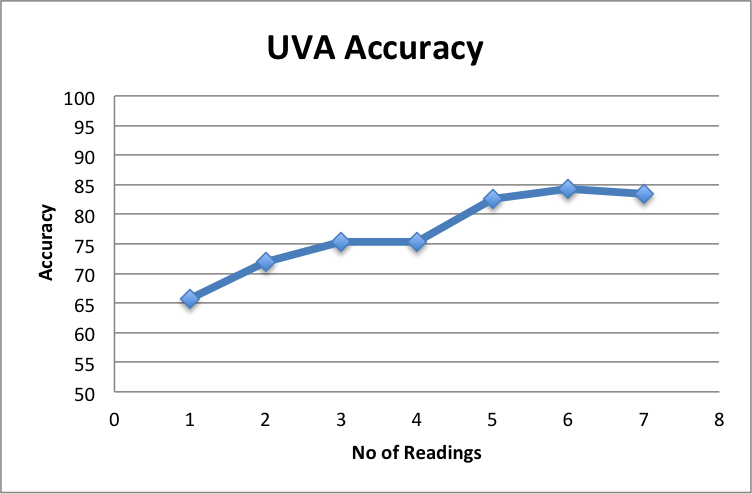
\includegraphics[scale=0.5]{segment4uva.png}
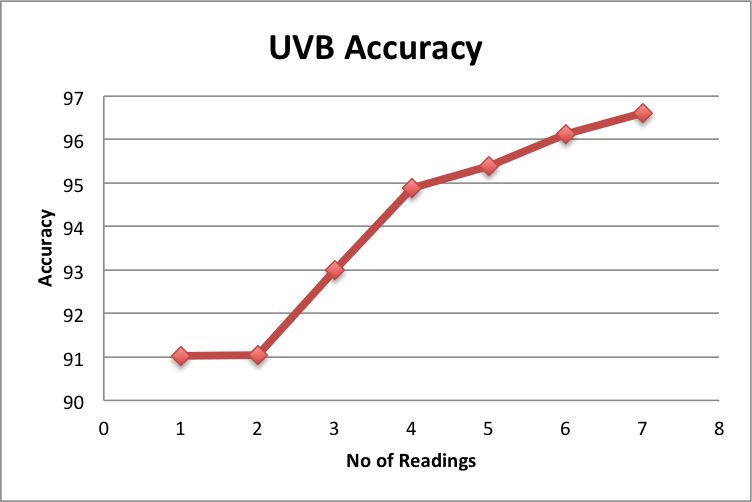
\includegraphics[scale=0.5]{segment4uvb.png}
\caption{\small \sl Accuracy v/s No of Readings for UVB}
\label{fig:lessReadings}
\end{center}
\end{figure}


As observed from the table \ref{seg4accuracy} that UVA takes 3 samples to reach the accuracy of 75\% and UVB take 4 readings to reach the accuracy of 95\%. 
\newpage\newpage
\begin{center}
Segment 5 as seen in Fig. ~\ref{fig:segment5}. \\
Start Point:  34.061717,-118.448455\\
End Point:  34.062535,-118.449184 \\
Total length of the segment was 480 ft.\\
Time of Day: Between 9am and 10am\\
\begin{figure}[h]
\begin{center}
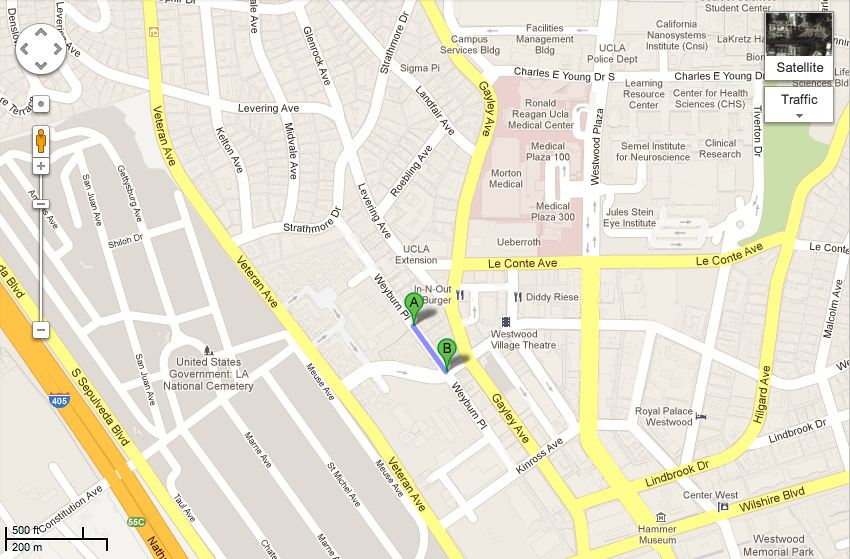
\includegraphics[scale=0.32]{segment5a.png}
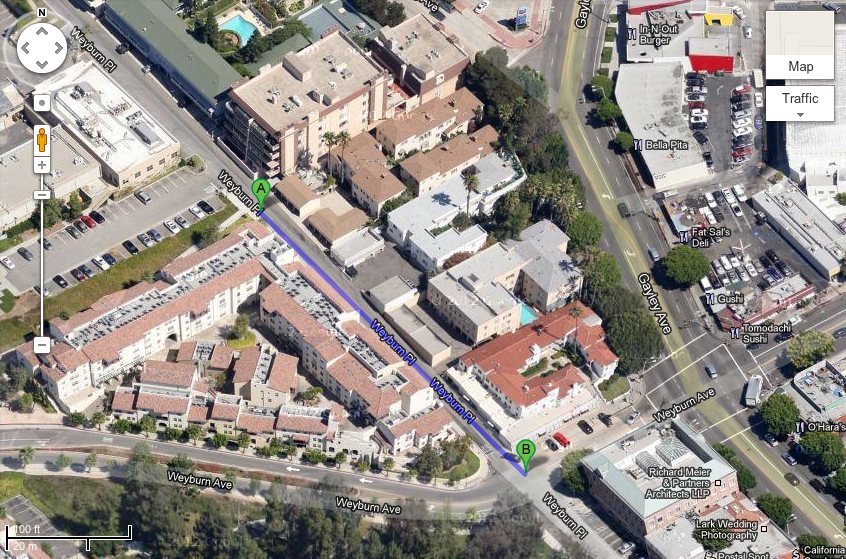
\includegraphics[scale=0.32]{segment5b.png}
\caption{\small \sl Sample selected segment map view}\label{fig:segment5}
\end{center}
\end{figure}
\end{center}
\newpage
\begin{table}
\centering
\begin{tabular}{|c|c|c|}
\hline
No of Readings & UVA Accuracy & UVB Accuracy \\
\hline 
1 & 69.59812 & 95.60988\\
\hline
2 & 78.61146 & 98.00997\\
\hline
3 & 87.20315 & 97.4513\\
\hline
4 & 90.96039 & 97.66619\\
\hline
5 & 92.75761 & 98.88199\\
\hline
6 & 88.489 & 98.63385\\
\hline
7 & 88.63886 & 98.75971\\
\hline
\end{tabular}
\caption{\small \sl Accuracy table for bootstraping}\label{seg5accuracy}
\end{table}


\begin{figure}
\begin{center}
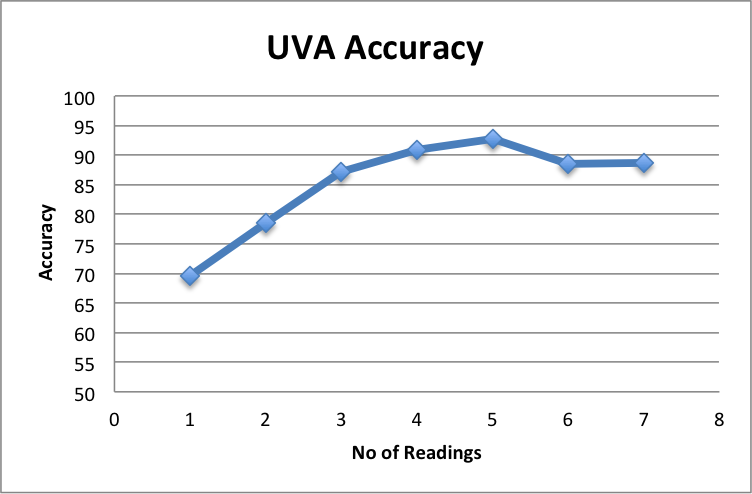
\includegraphics[scale=0.5]{segment5uva.png}
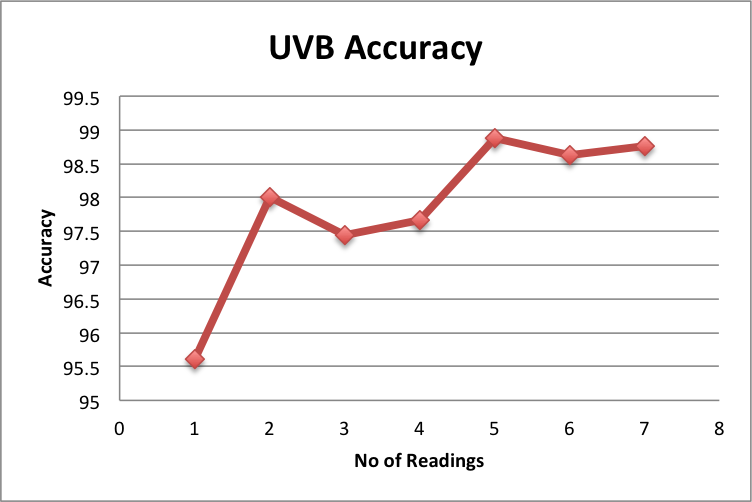
\includegraphics[scale=0.5]{segment5uvb.png}
\caption{\small \sl Accuracy v/s No of Readings for UVB}
\label{fig:lessReadings}
\end{center}
\end{figure}


As observed from the table \ref{seg5accuracy} that UVA takes 2 samples to reach the accuracy of 75\% and UVB take 1 readings to reach the accuracy of 95\%. 
\newpage\newpage
\begin{center}
Segment 6 as seen in Fig. ~\ref{fig:segment6}. \\
Start Point:  34.06197,-118.447984\\
End Point:  34.062575,-118.448217 \\
Total length of the segment was 226 ft.\\
Time of Day: Between 9am and 10am\\
\begin{figure}[h]
\begin{center}
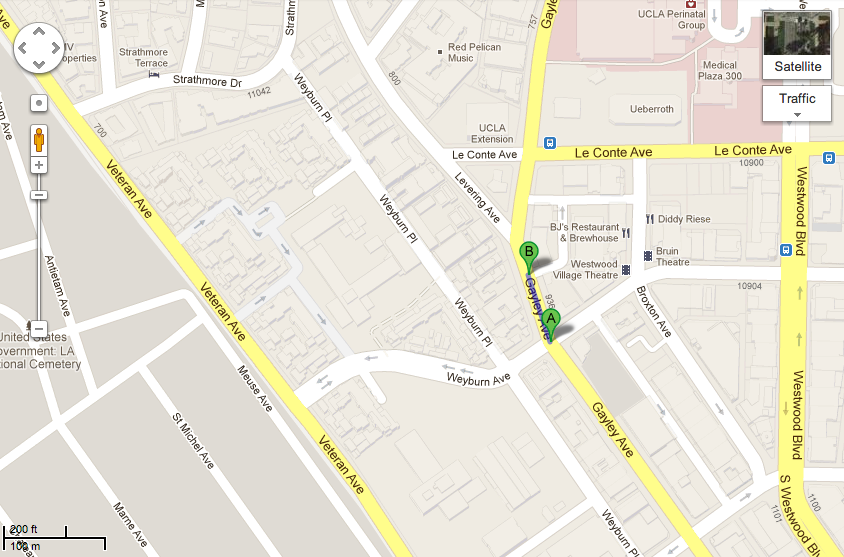
\includegraphics[scale=0.32]{segment6a.png}
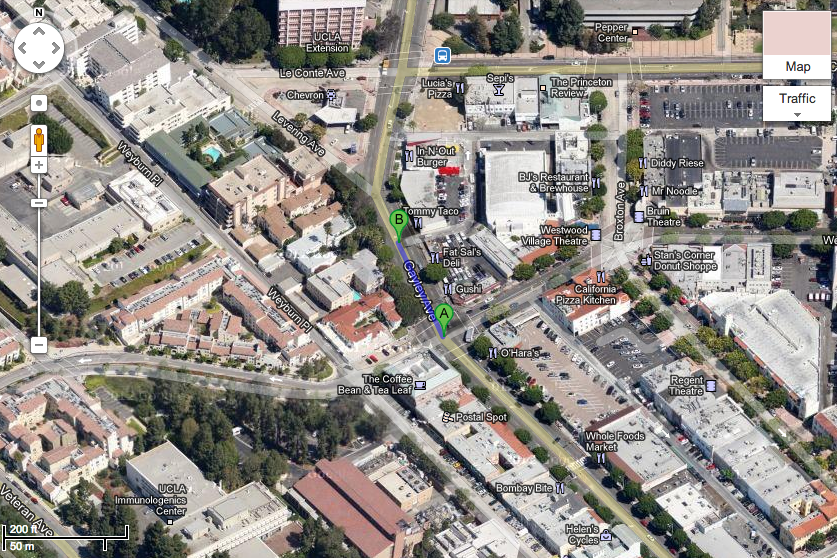
\includegraphics[scale=0.32]{segment6b.png}
\caption{\small \sl Sample selected segment map view}\label{fig:segment6}
\end{center}
\end{figure}
\end{center}
\newpage
\begin{table}
\centering
\begin{tabular}{|c|c|c|}
\hline
No of Readings & UVA Accuracy & UVB Accuracy \\
\hline 
1 & 71.31901 & 92.55076\\
\hline
2 & 81.64635 & 94.07683\\
\hline
3 & 87.95883 & 97.4513\\
\hline
4 & 91.56362 & 96.77067\\
\hline
5 & 96.39601 & 98.60045\\
\hline
6 & 95.10367 & 97.80031\\
\hline
7 & 98.67633 & 98.67633\\
\hline
\end{tabular}
\caption{\small \sl Accuracy table for bootstraping}\label{seg6accuracy}
\end{table}


\begin{figure}
\begin{center}
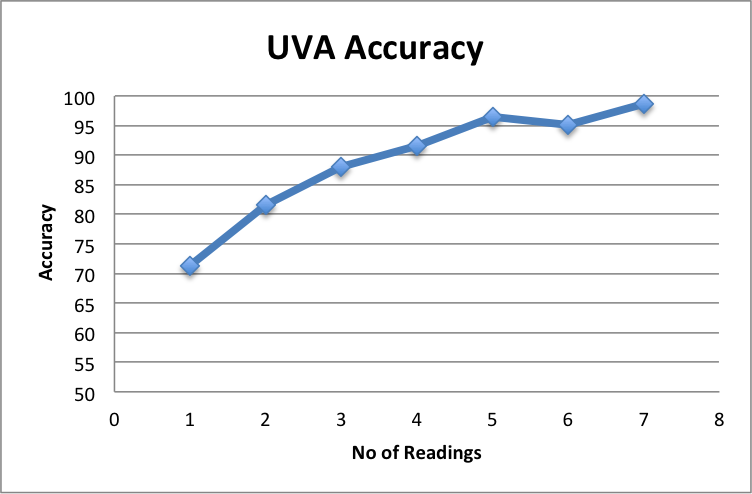
\includegraphics[scale=0.5]{segment6uva.png}
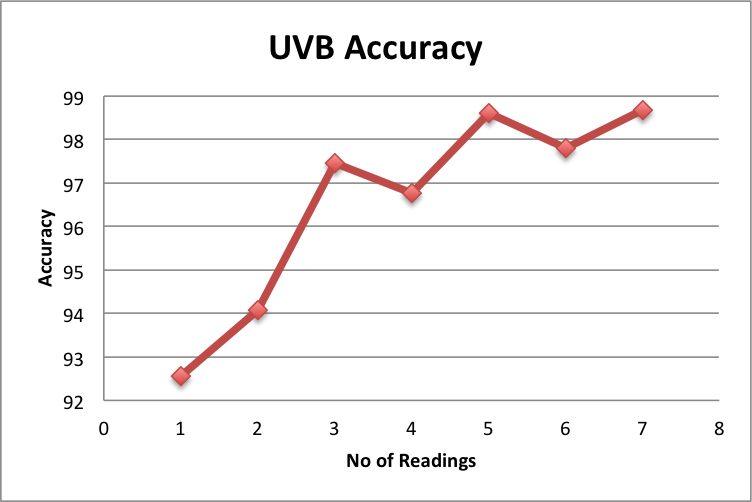
\includegraphics[scale=0.5]{segment6uvb.png}
\caption{\small \sl Accuracy v/s No of Readings for UVB}
\label{fig:lessReadings}
\end{center}
\end{figure}


As observed from the table \ref{seg6accuracy} that UVA takes 2 samples to reach the accuracy of 75\% and UVB take 3 readings to reach the accuracy of 95\%. 
\newpage\newpage
\begin{center}
Segment 7 as seen in Fig. ~\ref{fig:segment7}. \\
Start Point:  34.064308,-118.451878\\
End Point:  34.064259,-118.451419\\
Total length of the segment was 180 ft.\\
Time of Day: Between 9am and 10am\\
\begin{figure}[h]
\begin{center}
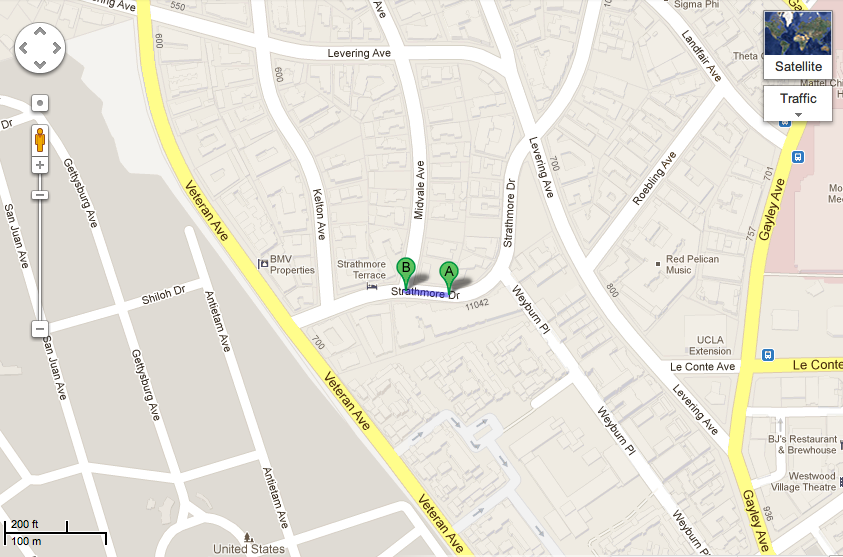
\includegraphics[scale=0.32]{segment7a.png}
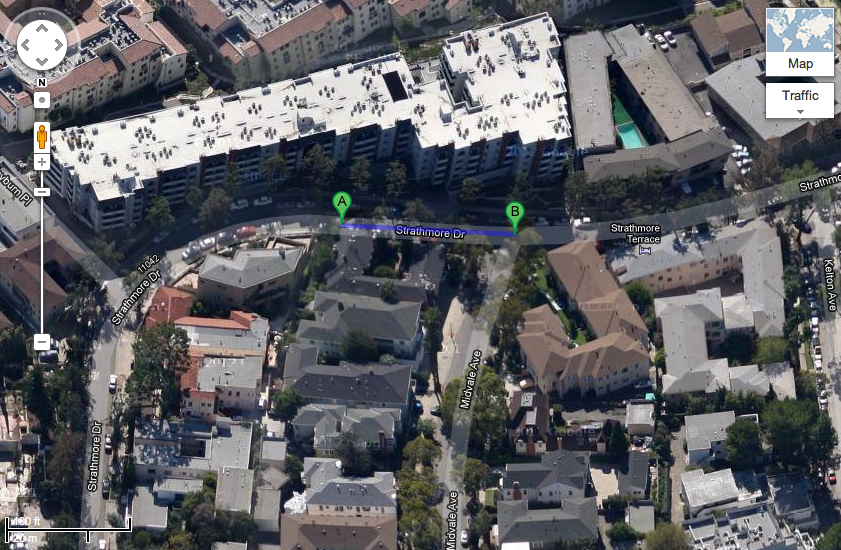
\includegraphics[scale=0.32]{segment7b.png}
\caption{\small \sl Sample selected segment map view}\label{fig:segment7}
\end{center}
\end{figure}
\end{center}
\newpage
\begin{table}
\centering
\begin{tabular}{|c|c|c|}
\hline
No of Readings & UVA Accuracy & UVB Accuracy \\
\hline 
1 & 65.80804 & 94.09919\\
\hline
2 & 72.6942 & 92.74988\\
\hline
3 & 78.4838 & 94.06129\\
\hline
4 & 85.92444 & 95.666\\
\hline
5 & 89.87737 & 96.45172\\
\hline
6 & 92.88613 & 96.82911\\
\hline
7 & 91.17483 & 97.67854\\
\hline
\end{tabular}
\caption{\small \sl Accuracy table for bootstraping}\label{seg7accuracy}
\end{table}


\begin{figure}
\begin{center}
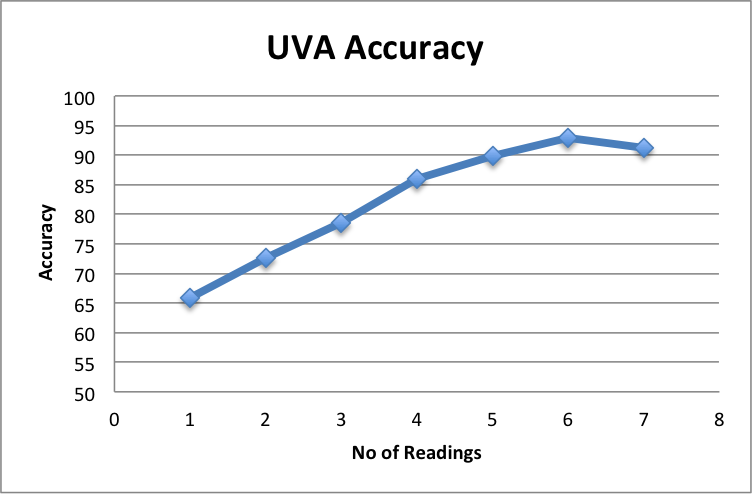
\includegraphics[scale=0.5]{segment7uva.png}
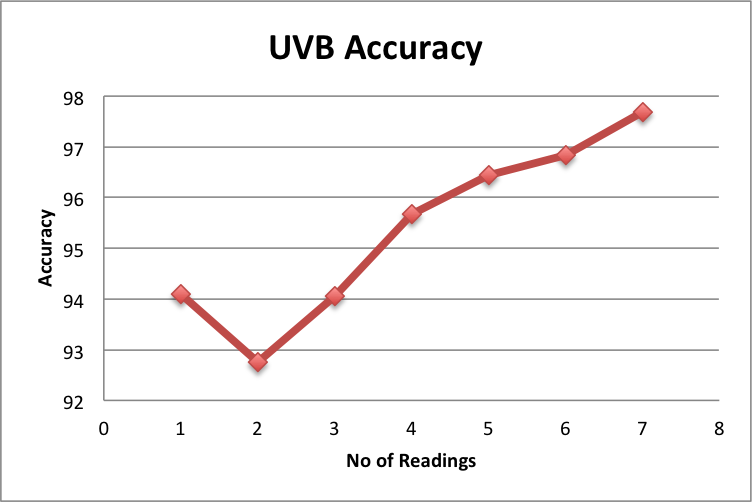
\includegraphics[scale=0.5]{segment7uvb.png}
\caption{\small \sl Accuracy v/s No of Readings for UVB}
\label{fig:lessReadings}
\end{center}
\end{figure}


As observed from the table \ref{seg7accuracy} that UVA takes 3 samples to reach the accuracy of 75\% and UVB take 4 readings to reach the accuracy of 95\%. 
\newpage


\newpage
After repeating this experiment for many different segments, observation was made that in the worst case, 6 points on a segment are necessary to get accuracy above 75\% for UVA and 4 points on a segment are necessary to get accuracy above 95\% for UVB.
In average case, 4 points on a segment are necessary to get accuracy above 75\% for UVA and  3 points on a segment are necessary to get accuracy above 95\% for UVB.


\subsubsection{Devising a method to handle segments with less number of samples than minimum required}
There may be some segments, which may not have the minimum number of readings that is necessary to assert the UV values like the segment in the Figure ~\ref{fig:lessReadings}. 
\begin{figure}
\begin{center}
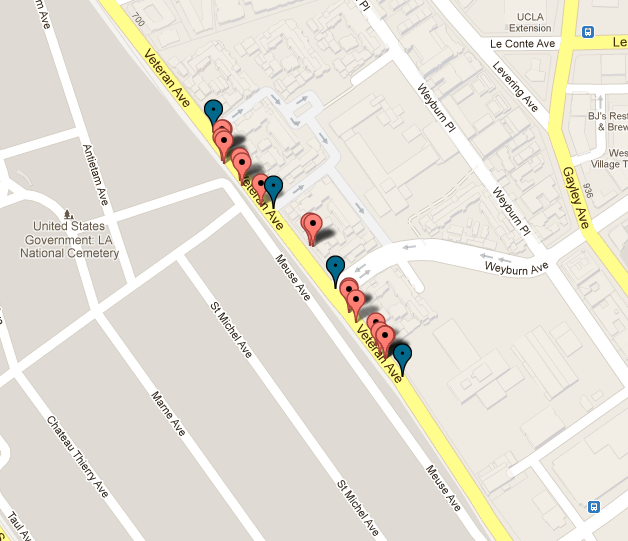
\includegraphics[scale=0.35]{lessReadings.png}
\caption{\small \sl Segment with less readings than minimum required}
\label{fig:lessReadings}
\end{center}
\end{figure}
The problem of some segments not having desired number of readings is countered in the way mentioned below. In that case, a weighted average of the readings from the neighboring segments is taken. The weight is in terms of how far the segment is from the segment, which is currently under consideration and also, the number of readings that the current segment has. The immediately neighboring segments have a weight of 0.5, the weight is decreased by 0.1 as segments farther from the segment under consideration is taken into account for calculating the UV values. This method was selected since segments, which are near the segment under consideration, have a high correlation of readings with the segment. The window of neighboring segments is expanded till the desired number of readings for the segment is achieved. 

For instance, if the segments in Figure ~\ref{fig:lessReadings} is considered. The segements end points are marked by blue colored markers and the red color markers indicate readings at those points. As observed in the figure, the number of readings are less than the minimum number of readings required. So, a weighted average of the neighboring segments is taken. Since both the segments are immediate neighbors, weight would eventually be proportional to the number of readings in each segment as there would be more confidence in considering readings from the segment that has more readings as compared to considering the segments with less number of readings. 

\newpage
\subsection{Web Service Developement}
Web Service was developed to provide API to the developers to make use of the common platform and develop navigation applications based in UV data. The Web Service developed is similar to the Google Maps Web Service \cite{googleWebService} with extra information about the UV levels along the route. Initially, data is pulled from Google Maps where information about routes, distance between the source and destination, time to travel and most importantly alternate route information is pulled. After parsing the information, we get the alternate routes i.e. the {\it legs}. For each {\it leg}, information about {\it steps} in each route is also retrived from Google Maps API. For each {\it step}, Open Street Maps API is called to get the segments inside each step. Then, UV data about each segment is retrieved from the database. After calculating the UV levels on each of the paths, an output of a path with minimum UV levels is passed to the caller. Thus, data from Google Maps is joined with data from Open Street Maps and joined with the UV data on a path and returned to the caller. A choice was to be made whether to display the output in XML format or JSON. Finally, the output was in JSON format since its easier to read. Its also less decoding effort to programmers as compared to XML output. The inputs to the web service are source latitude, source longitude, destination latitude, destination longitude and UV criteria. UV criteria is whether route with minimum UVA or minimum UVB or an average of UVA and UVB is required. A part of sample output from the webservice is in Fig 
\ref{fig:webServiceOutput}
\begin{figure}[h]
\begin{center}
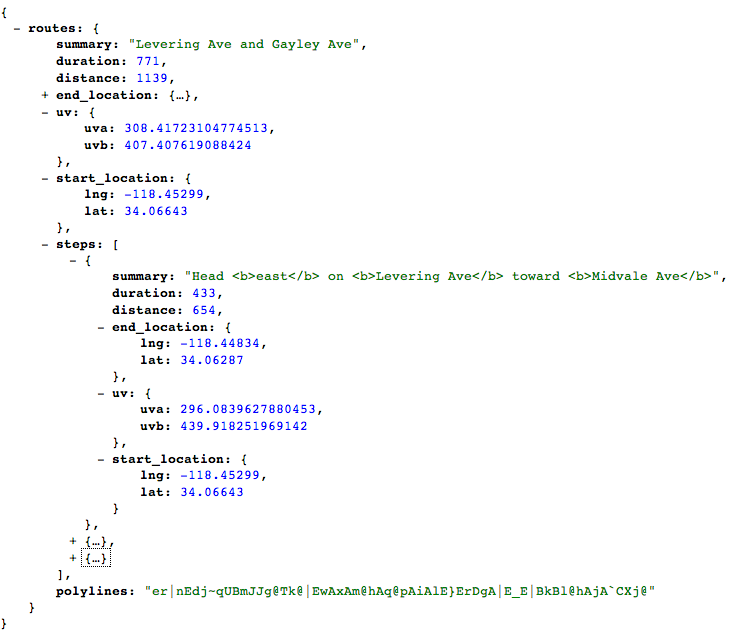
\includegraphics[scale=0.4]{webServiceOutput.png}
\caption{\small \sl Sample Web Service Output}
\label{fig:webServiceOutput}
\end{center}
\end{figure}
\clearpage

\newpage
\subsection{Navigation Web Application}
A Web Application is built in order to consume the web service built. The purpose of the web application is to serve as a basis for developers to use the system and build applications on top of it. The web application shown in Fig \ref{sampleWebApplication} is built using the web service and google maps javascript API to render the maps on the web page. Similarly other desktop and mobile applications can also be built. When entered the source and destination latitude and longitude and selecting the UV criteria, the application will suggest the most optimum route based upon the selected criteria as showin in Fig \ref{fig:webapp}.
\begin{figure}[ht]
\begin{center}
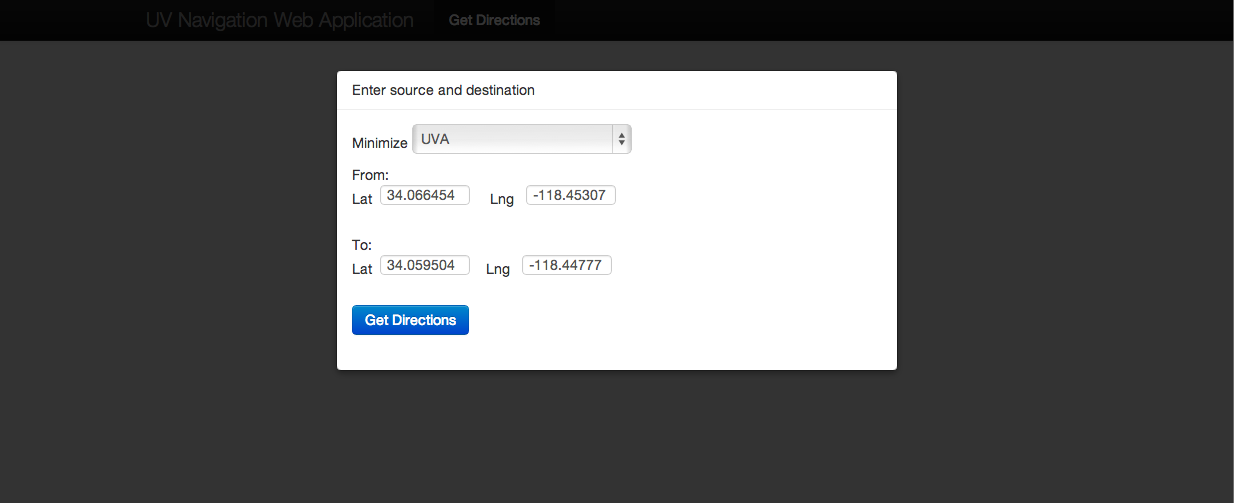
\includegraphics[scale=0.30]{webapp1.png}
\caption{\small \sl a. UV Navigation Web Application }
\label{fig:webapp}
\end{center}
\end{figure}
\begin{figure}[ht]
\begin{center}
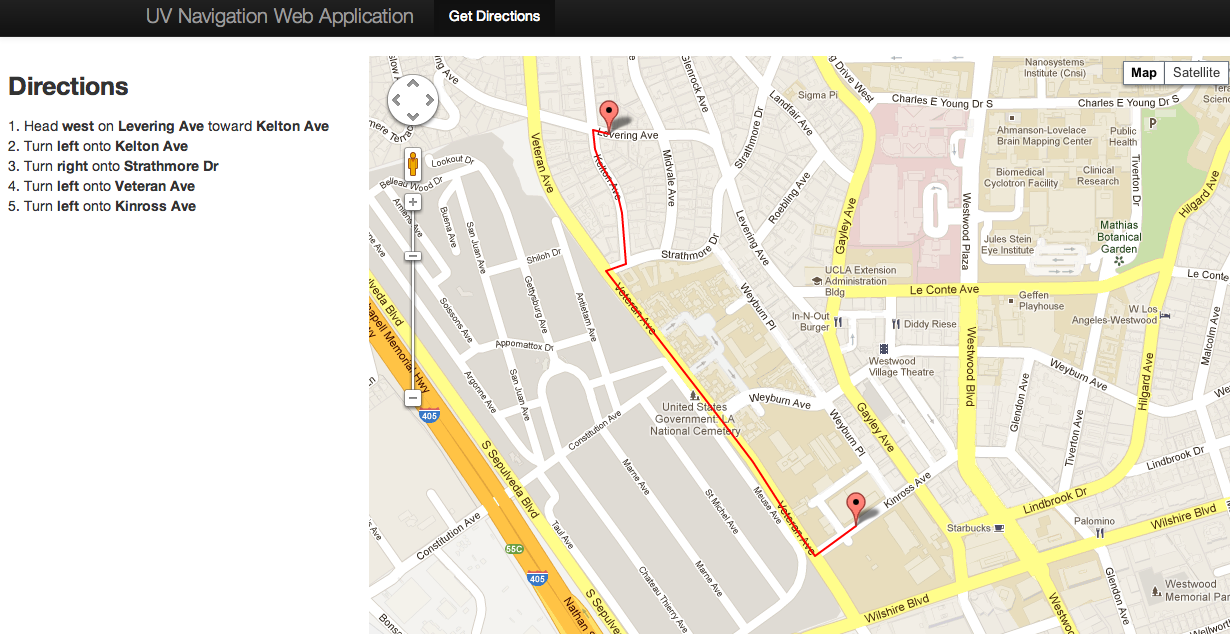
\includegraphics[scale=0.35]{webapp2.png}
\caption{\small \sl b. UV Navigation Web Application }
\label{fig:webapp}
\end{center}
\end{figure}
\clearpage
\newpage
\section{Experiment}
Taking the results from the data analysis that was done, experiments were performed to verify whether the desired accuracy was achieved. As per the observations from the data analysis,in the worst case, 6 points on a segment are necessary to get accuracy above 75\% for UVA and 4 points on a segment are necessary to get accuracy above 95\% for UVB.
In average case, 4 points on a segment are necessary to get accuracy above 75\% for UVA and  3 points on a segment are necessary to get accuracy above 95\% for UVB. The best possible approach to test the analysis was to randomly take the number of sample points actually necessary and check whether the desired accuracy is achieved. To remove the randomness from the process, sample number of points were taken around 100 times and their accuracy was calculated. This accuracy was verified with the desired accuracy. 

\lstset{ tabsize=4,      caption=R Code for verifying accuracy,breaklines=true,
        frame=single}
\begin{lstlisting}
route <- read.csv("route.txt", header=TRUE  , sep=",")
sampleSet = 4 # for worst case scenario
uvb = route$uvb # get UVB values
uvbAccuracy <- vector()
for(i in 1:100){
  uvbSample = sample(uvb,sampleSet)
  trueMean = mean(route5$uvb)
  sampleMean = mean(uvbSample)
  t = abs(100-abs((trueMean-sampleMean)/ sampleMean*100))
  uvbAccuracy[i]=t
  }
\end{lstlisting}

Again, some segments were selected. Accuracy was determined by considering the worst case as well as average case scenario. The results were as follows for different segments of the road. \\
\newpage
\begin{table}[h]
\centering
\begin{tabular}{|c|c|c|c|c|c|}
\hline
&&UVA & UVB \\ 
\hline
Route 1 & Average Case & 75.93203 & 96.50077 \\\cline{2-4}
&  Worst Case & 79.50551 &  96.74856\\\cline{2-4}
\hline 
Route 2 & Average Case & 74.38072 & 96.12223 \\\cline{2-4}
&  Worst Case & 81.07674 &  96.06205\\\cline{2-4}
\hline 
Route 3 & Average Case & 81.29109 & 95.44681 \\\cline{2-4}
&  Worst Case & 87.52028 &  95.89465\\\cline{2-4}
\hline 
Route 4 & Average Case & 88.40942 & 95.25212 \\\cline{2-4}
&  Worst Case & 91.58414 &  95.81699\\\cline{2-4}
\hline 
Route 5 & Average Case & 83.29114 &  97.71054 \\\cline{2-4}
&  Worst Case & 88.49399 &  98.27896\\\cline{2-4}
\hline 
Route 6 & Average Case & 92.15421 & 96.50476 \\\cline{2-4}
&  Worst Case & 95.55486 &  97.02755\\\cline{2-4}
\hline 
Route 7 & Average Case & 89.63042 & 94.82353 \\\cline{2-4}
&  Worst Case & 91.7044 &  96.18621\\\cline{2-4}
\hline 

\end{tabular}
\caption{\small \sl Experiment Results}\label{exp}
\end{table}

From the obersvation in table \ref{exp} of all the readings, it could be inferred that if 6 samples to estimate UVA and 4 to estimate UVB are taken, then the accuracy remains above the thresholds that are required.
\newpage

\section{Future Work}
The work can be extened to do analysis on different paths. That way, the current number of samples of can be reaffirmed. Since the accuracy of UVA is aimed to be 75\%, a more accurate UVA sensor could be used and a higer UVA accuracy could be aimed for. The current accuracy limits are selected from \cite{uvguardian} since extensive research was done and also the sensor used was the same one as used in this experiment. UV sensors could be interfaced directly with the android device which could facilitate more flexibilty to gather data. After that is achieved, more users could be encouraged to gather UV data. In this way, crowd sourcing could be used to populate the database eventually helping uses navigate more routes.
\newpage
\section{Conclusion}
It could be concluded that in the worst case, 6 points on a segment are necessary to get accuracy above 75\% for UVA and 4 points on a segment are necessary to get accuracy above 95\% for UVB. In average case, 4 points on a segment are necessary to get accuracy above 75\% for UVA and  3 points on a segment are necessary to get accuracy above 95\% for UVB. The number of points on a segment is not dependend on the length of the segment since the length of the segments are generally small. A web service was developed to estimate UV levels on a path and route the user through the path having the minimum UV value.

\newpage
\begin{thebibliography}{6}
\bibitem{dep1} M. Nathaniel Mead, Benefits of Sunlight: A Bright Spot for Human Health
\bibitem{dep2} Richard H. Grant and Gordon M. Heisler, Effect of Cloud Cover on UVB Exposure Under Tree Canopies: Will Climate Change Affect UVB Exposure? 
\bibitem{dep3}Richard H. Grant , Gordon M. Heisler and Wei Gao, Estimation of Pedestrian Level UV Exposure Under Trees
\bibitem{dep4} http://articles.mercola.com/sites/articles/archive/2012/03/26/maximizing-vitamin-d-exposure.aspx
\bibitem{dep5} Wong, C.F., Toomey, S., Fleming, R.A., Thomas, B.W., 1995, UV-B radiometry and dosimetry for solar measurements, Journal of the Health Physics Society,Vol. 68.
\bibitem{uvguardian}Jerrid Matthews, Farnoosh Javadi, Gauresh Rane, Jason Zheng, Giovanni Pau, Mario Gerla, Ultraviolet Guardian - Real Time Ultraviolet Monitoring
\bibitem{googleMapsOriginal} http://maps.google.com
\bibitem{googleWebService}https://developers.google.com/maps/documentation/directions/
\bibitem{openStreetMap}http://www.openstreetmap.org/
\bibitem{openStreetMapsDirections}http://wiki.openstreetmap.org/wiki/YOURS

\end{thebibliography}


\end{document}